\chapter{Results}\label{chapt:results}

With so much to talk in this report, everything can be summarised into a small picture - \cref{fig:the_complete_picture}.

% \section{Pros}
The model predicted most of the roads, which were predicted by the model without super-resolution. Apart from that, the model also predicted a lot of other small roads. On validating with the ground truth images, I found that this was a very good prediction. Checkout \cref{fig:run_merge_road_maps}.

\begin{figure}[h!]
  \centering
  \begin{subfigure}{0.5\textwidth}
    \centering
    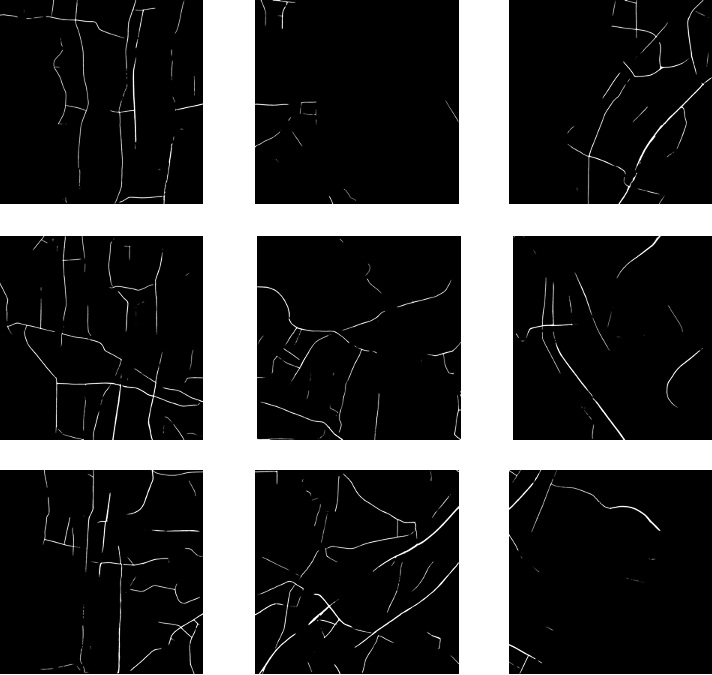
\includegraphics[width=\textwidth]{run_roads}
    \caption{}
  \end{subfigure}~
  \begin{subfigure}{0.5\textwidth}
    \centering
    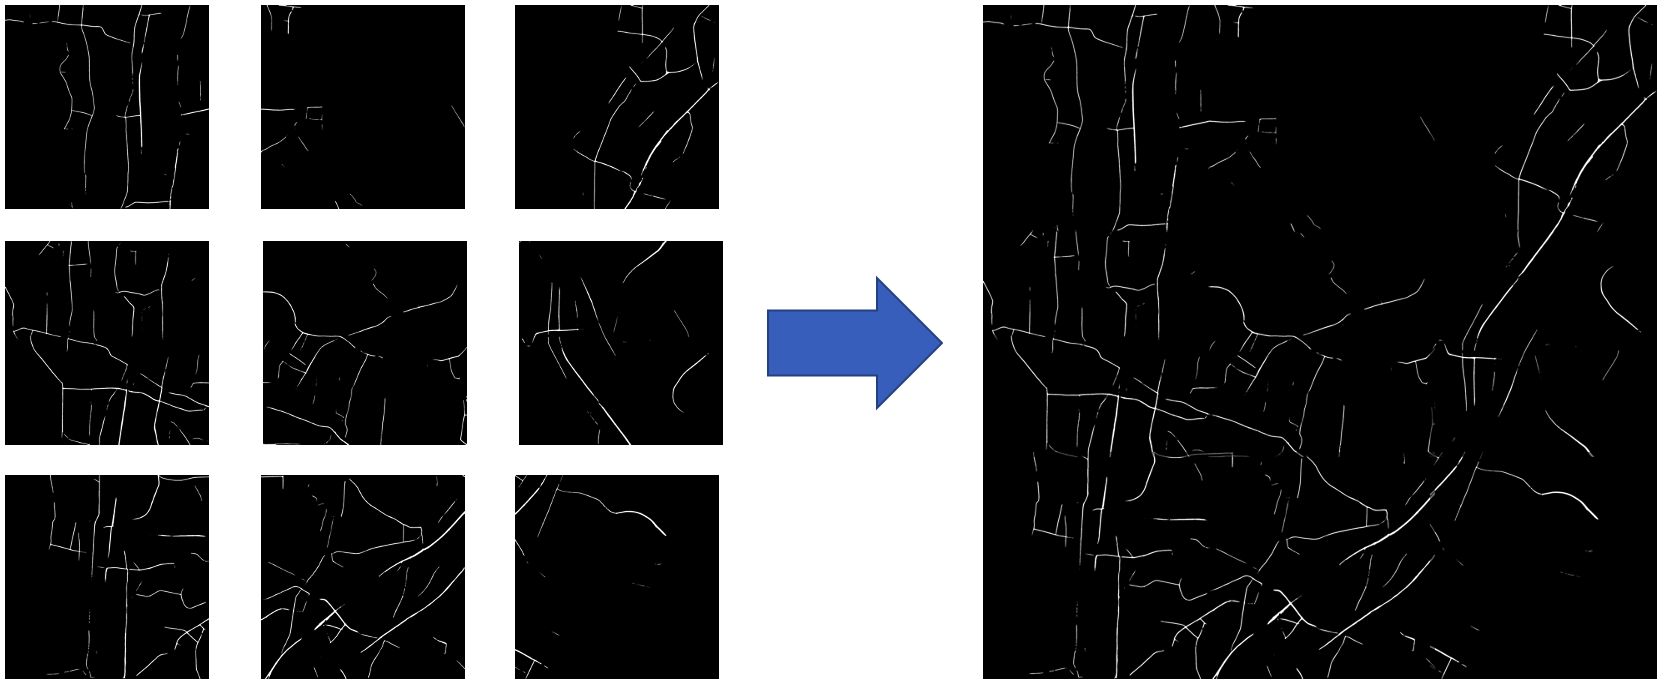
\includegraphics[width=0.96\textwidth]{run_merge_roads}
    \caption{}
  \end{subfigure}
  \begin{subfigure}{0.5\textwidth}
    \centering
    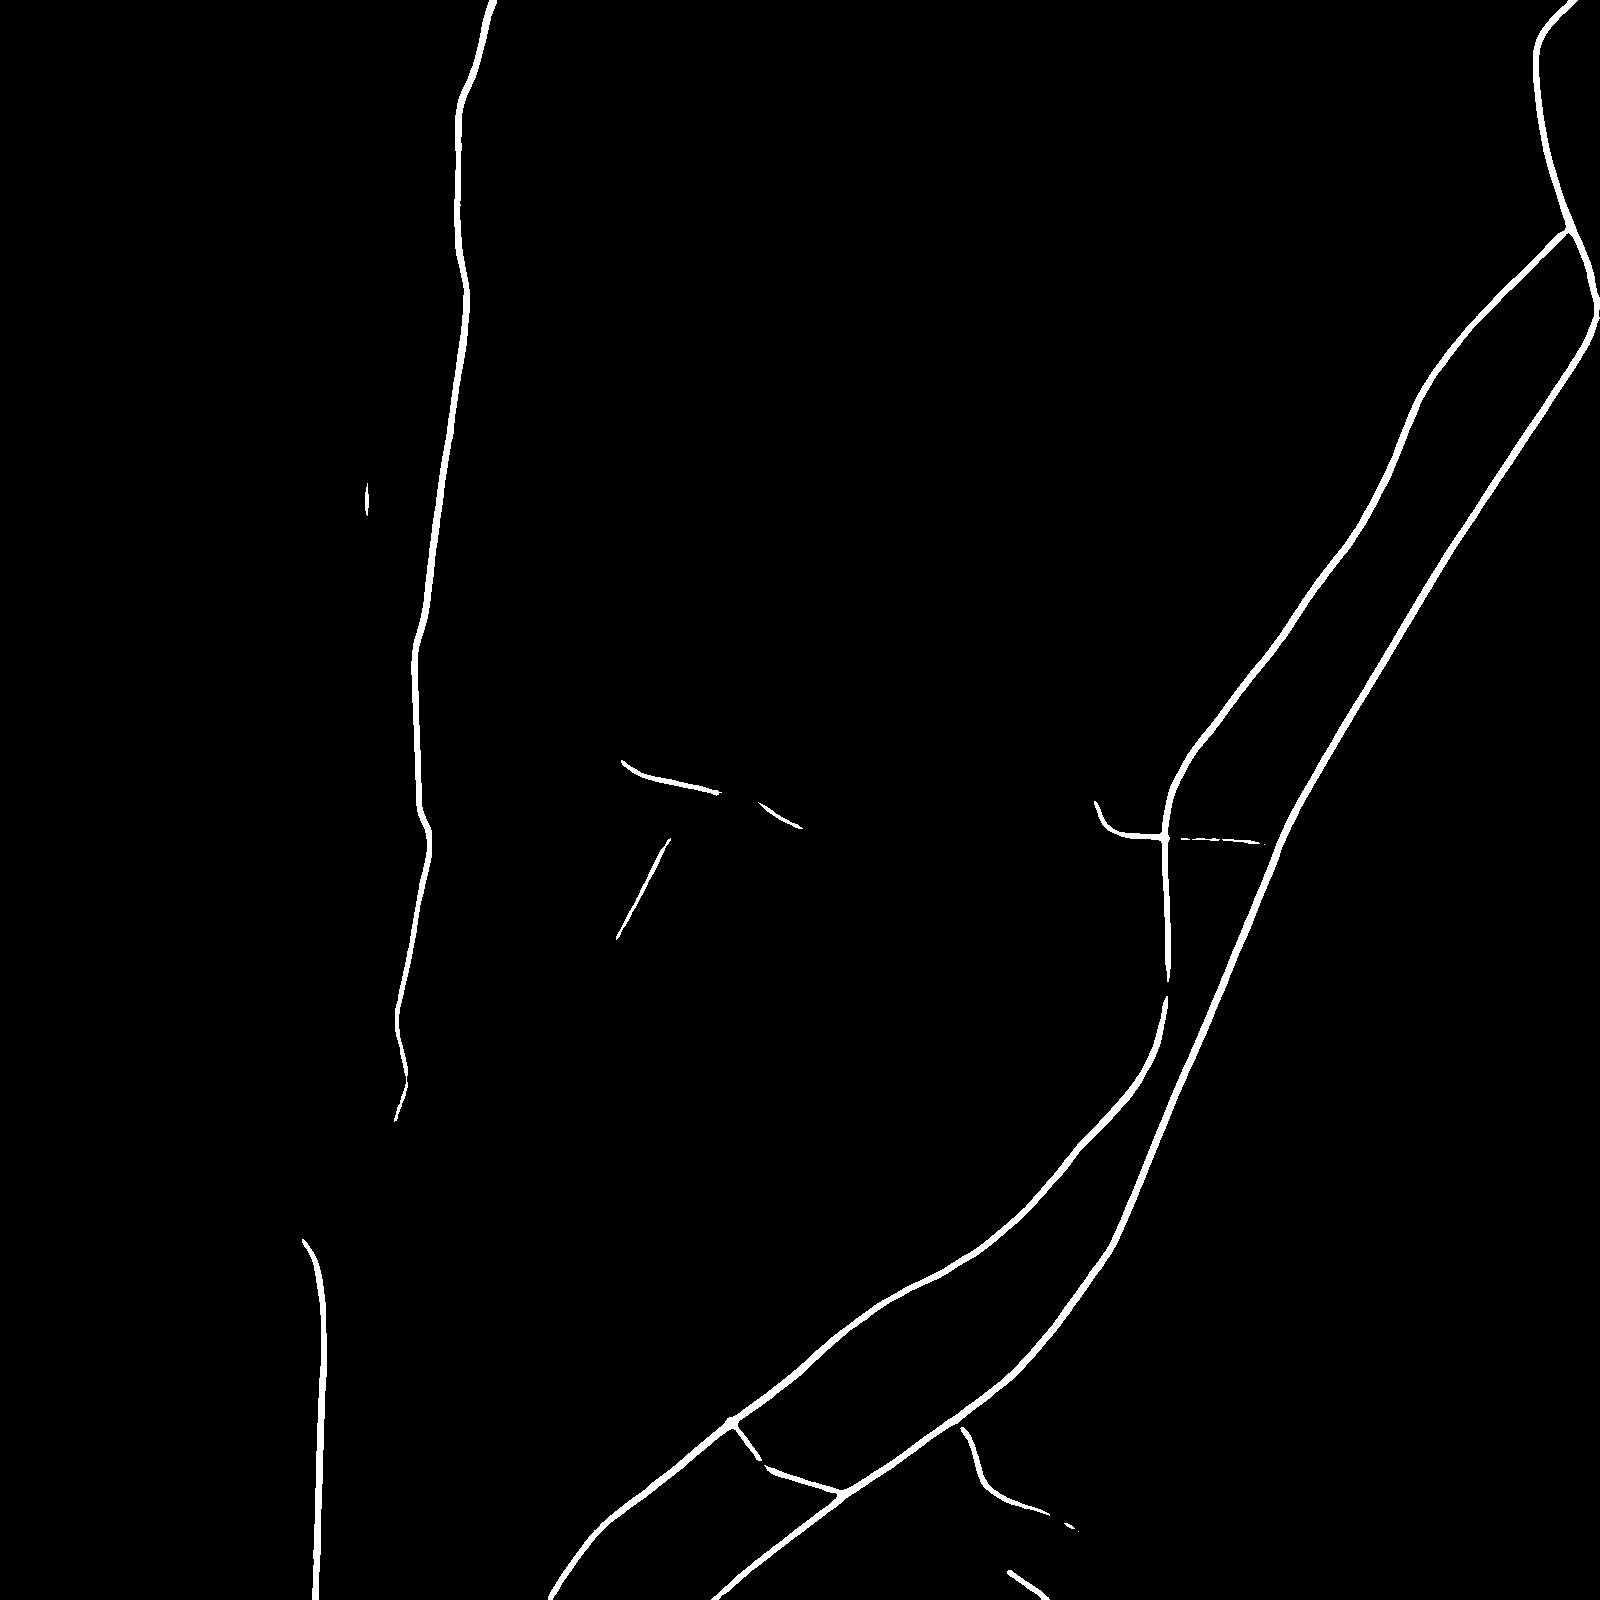
\includegraphics[width=\textwidth]{run_road_linknet}
    \caption{}
  \end{subfigure}~
  \begin{subfigure}{0.5\textwidth}
    \centering
    \includegraphics[width=\textwidth]{sat_image_run}
    \caption{}
  \end{subfigure}
  \caption[Predictions]{\textbf{(a)} Predictions using our model. \textbf{(b)} Merging the predictions \textbf{(c)} Predictions just using the road-detection model. \textbf{(d)} Image used to find predictions. Comparing the original road-detection model with the improved model.}
  \label{fig:run_merge_road_maps}
\end{figure}


% \section{Cons}
Though the prediction is a significant improvement, One of the most noticeable drawbacks of using this model is the amount of time required to get the predictions. 

Another disadvantage is, the model is too much affected due to inaccuracies in the training dataset. This is particularly visible for wide roads, say, an 8~lane road, on a 10~m resolution. As seen in \cref{fig:run_merge_road_maps}, the thick roads (the ones predicted in \textbf{(b)}) are seen to be lacking certain amount of continuity. The discontinuity is mainly because of the noise, which has affected the weights. This error can be reduced by training the model with more precise data. As obtaining precise data is an expensive operation, another way to correct this error to a certain extent is to run the algorithm without super-resolution and to average the results with appropriate weightage given to both road-detection `With super-resolution' and `Without super-resolution.'

Now that we have two predictions, one with super-resolution and without it, we merge them. First, we need to make them of the same resolutions. We do this by finding out the difference factor. Let us say the difference factor is $X$ on each side; we split the lower resolution image pixels into $X$ different pixels on both sides. Then we average the resultant images of the same resolution. For reference: look at \cref{fig:roads_in_confidence}.

\begin{figure}[h!]
  \begin{subfigure}[b]{0.25\textwidth}
    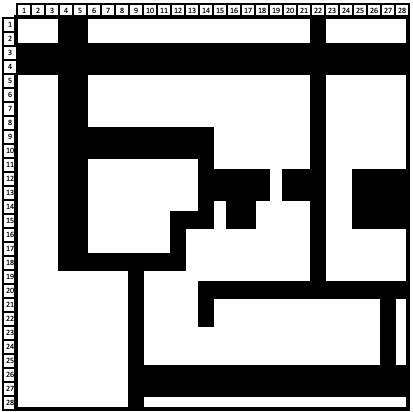
\includegraphics[width=\textwidth]{roads_with_SR}
    \caption{}
  \end{subfigure}~
  \begin{subfigure}[b]{0.15\textwidth}
    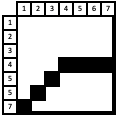
\includegraphics[width=\textwidth]{roads_without_SR}
    \caption{}
  \end{subfigure}~
  \begin{subfigure}[b]{0.25\textwidth}
    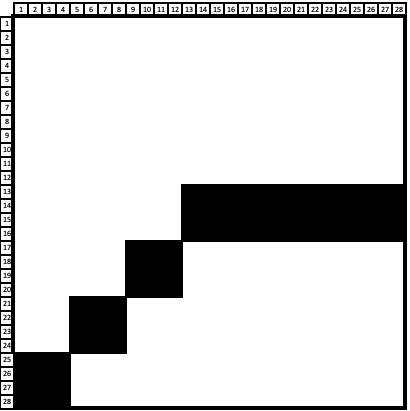
\includegraphics[width=\textwidth]{roads_without_SR_zoomed}
    \caption{}
  \end{subfigure}~
  \begin{subfigure}[b]{0.25\textwidth}
    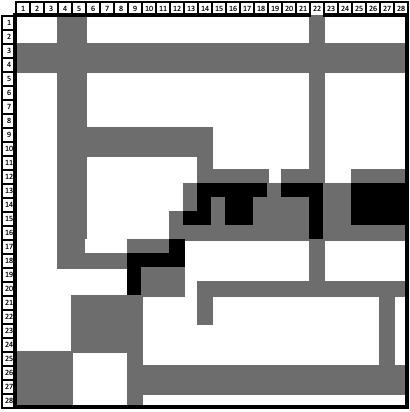
\includegraphics[width=\textwidth]{roads_with_confidence}
    \caption{}
  \end{subfigure}
  \caption[Finding likelihood of roads in predictions]{Merging roads found with \textbf{(a)} Predictions with SR. \textbf{(b)} Predictions without SR. \textbf{(c)} Upscaling of (b). \textbf{(d)} Final result by averaging (a) and (c). Black ones are definitely a road, grey ones having 0.5 probablity of being a road and least likely to find a road on the white pixel.}
  \label{fig:roads_in_confidence}
\end{figure}

\textbf{Note:} The model described in this complete report is strictly for mid-resolution satellite data. If the method is applied to macro images (such as an on-ground camera or an aerial image), the consequences can be disastrous. For example, look at (\cref{fig:cons_coverleaf}) where we used aerial image and applied our model.

\begin{figure}[h!]
  \centering
  \begin{subfigure}{0.3\textwidth}
    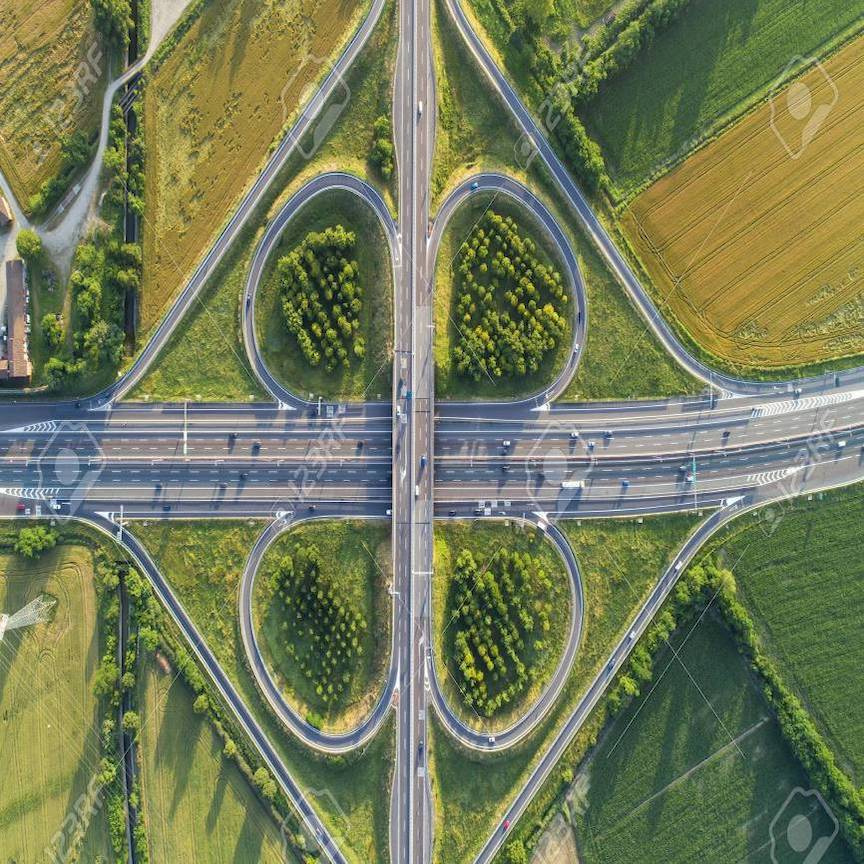
\includegraphics[width=\textwidth]{cons_coverleaf}
    \caption{}
  \end{subfigure}~
  \begin{subfigure}{0.3\textwidth}
    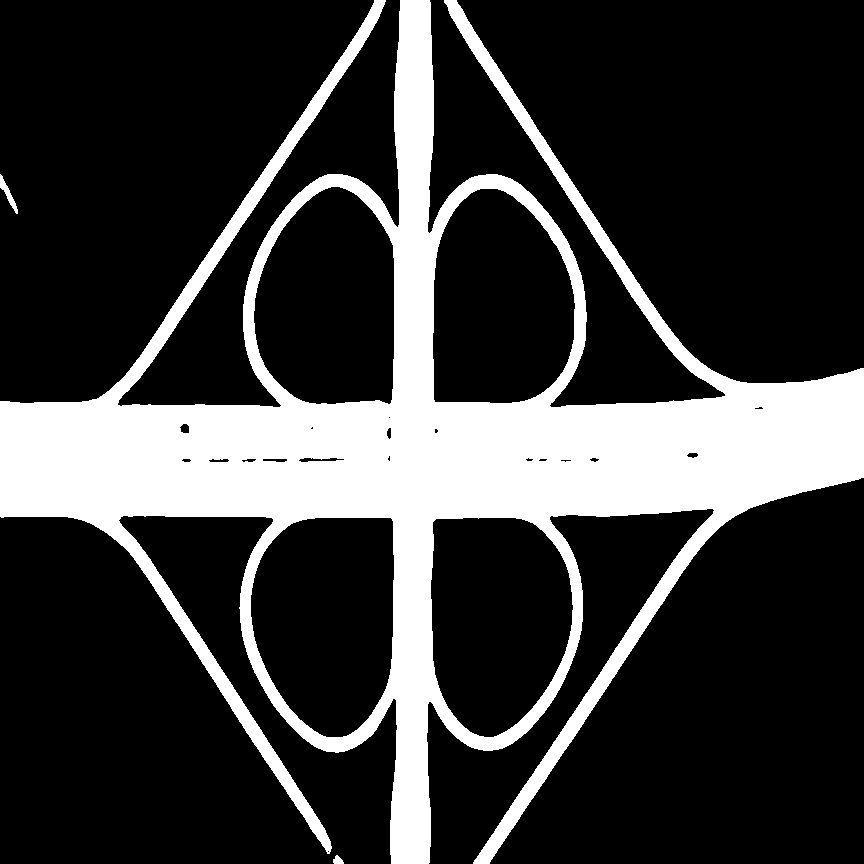
\includegraphics[width=\textwidth]{cons_road_coverleaf}
    \caption{}
  \end{subfigure}~
  \begin{subfigure}{0.3\textwidth}
    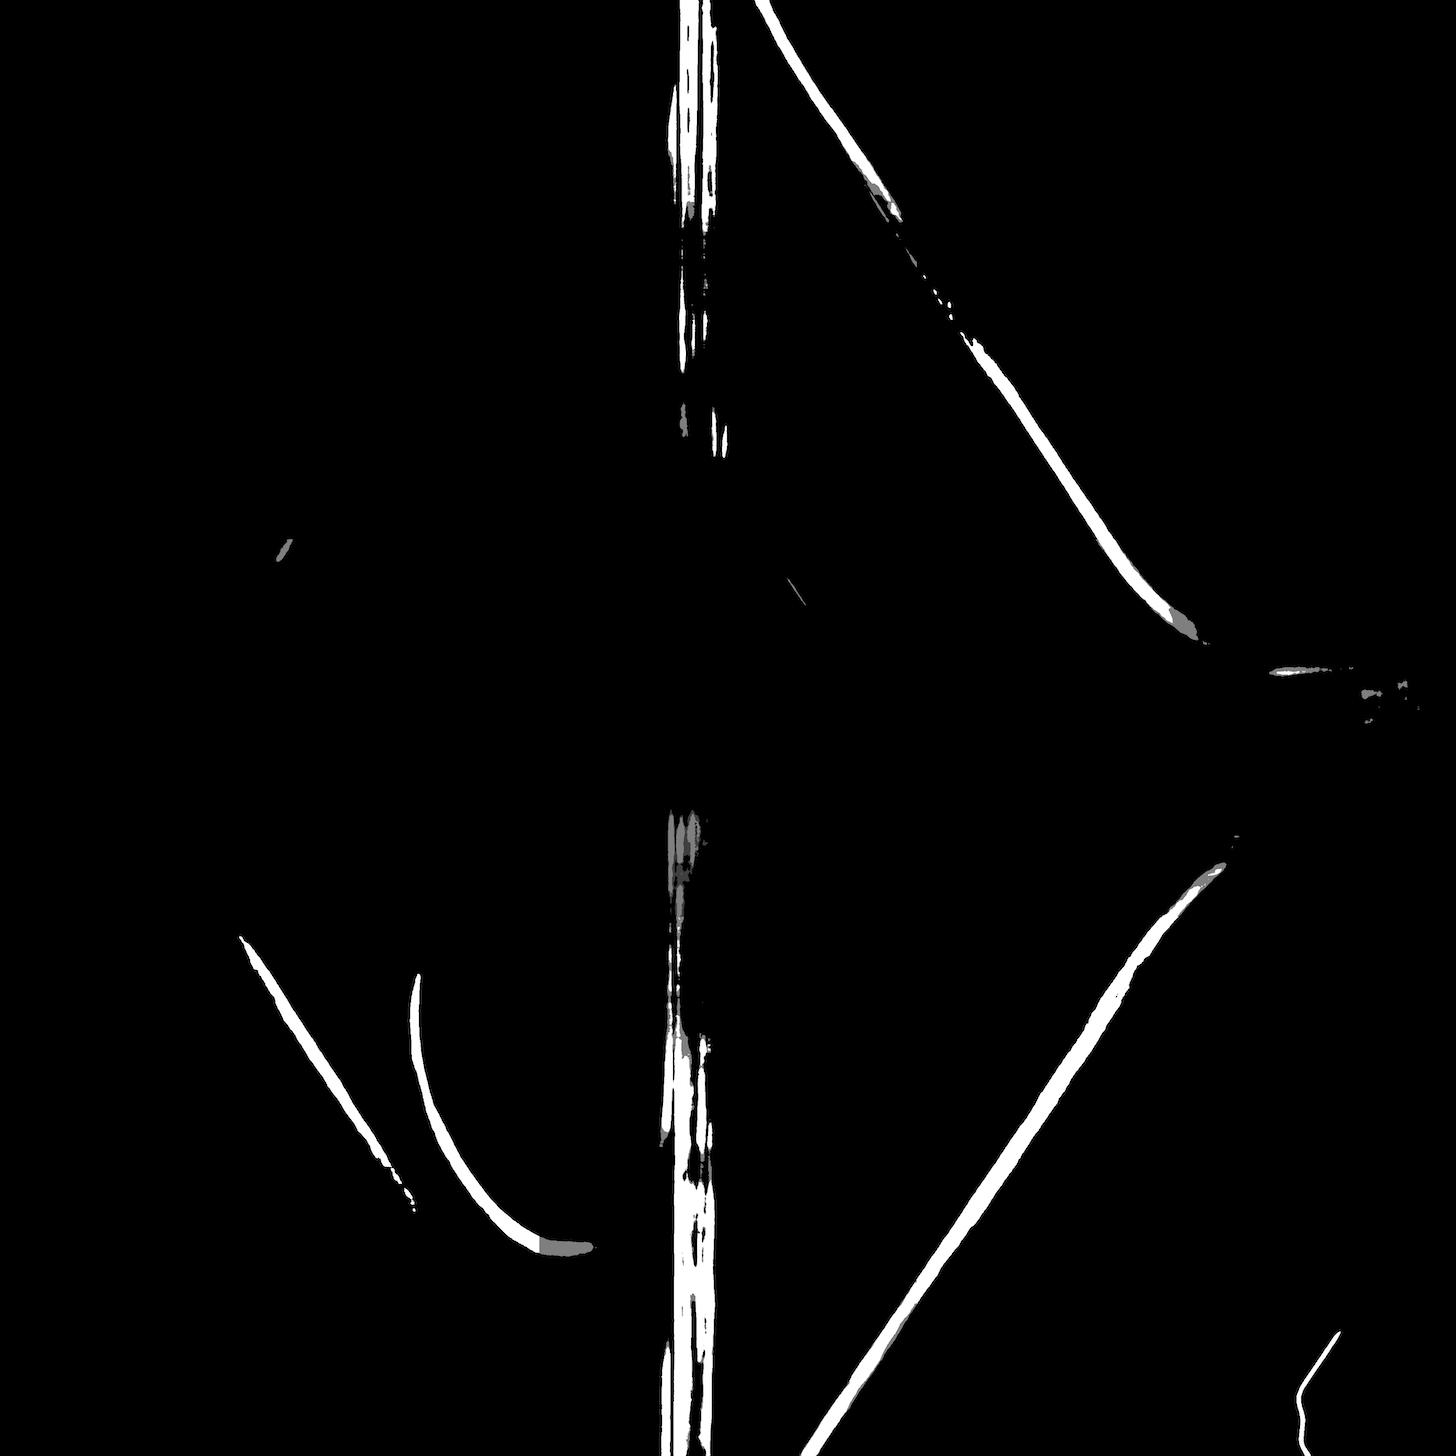
\includegraphics[width=\textwidth]{cons_road_coverleaf_sr}
    \caption{}
  \end{subfigure}
  \caption[Disastors in applying the model on unexpected images]{\textbf{(a)} The image to apply the model on. \textbf{(b)} Road detection without applying super-resolution. \textbf{(c)} Road detection by our model. Notice how the accuracy drops when we apply the model on an aerial image.}
  \label{fig:cons_coverleaf}
\end{figure}

\begin{sidewaysfigure}
  \centering
  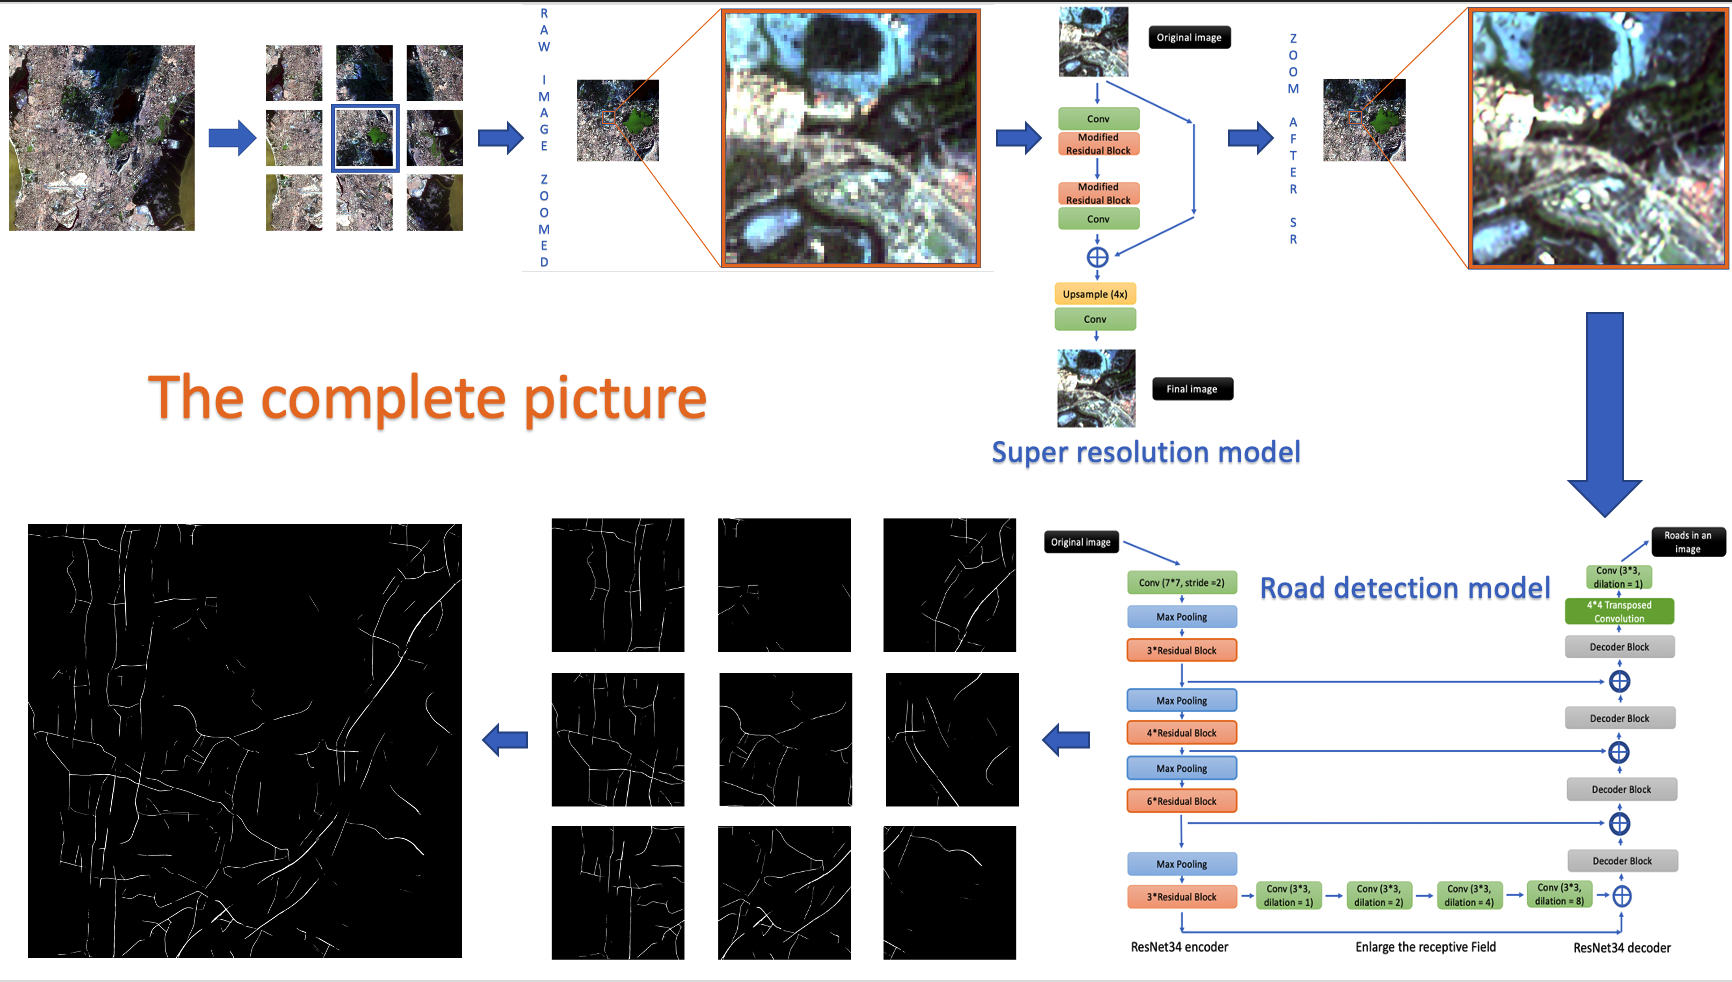
\includegraphics[width=\textheight]{the_complete_picture}
  \caption{A figure summarising the complete process into one.}
  \label{fig:the_complete_picture}
\end{sidewaysfigure}

% \chapter{Conclusions}
\chapter{Conclusions and Scope of Improvements}

Thanks to \href{https://arxiv.org/pdf/1805.06561.pdf}{DeepGlobe 2018: A Challenge to Parse the Earth through Satellite Images} and \href{http://openaccess.thecvf.com/content_cvpr_2018_workshops/papers/w4/Zhou_D-LinkNet_LinkNet_With_CVPR_2018_paper.pdf}{Submissions for the DeepGlobe Road Extraction Challenge}, I could test the hypothesis that indeed super-resolution can improve the results drastically.

In this process, we see that the narrow roads that were not recognized by the road-detection model are now visible in the predictions at the cost of the spatial connectivity of broad roads. Another significant observation is that the model is applied on broad roads. This is because the noise generated during super-resolution becomes much more dominant in monotonic features.

We see that super-resolution and road-detection both use Deep Convolution Neural Network. We train both the models separately and use them one after the other, to find significantly better results than any existing models. Now that the hypothesis that merging SR improves road-detection results is proven to be correct, the next step is making a single model that will detect roads instead of relying on two different models. This is logically feasible because both the models are DCNN, and another DCNN should replicate the behavior in a single model.

% https://towardsdatascience.com/road-segmentation-727fb41c51af
\pagebreak
